\documentclass[25pt,a0paper, portrait, colspace = 0.5cm, blockverticalspace = 5mm]{tikzposter}
\usepackage{blindtext}
\usepackage{comment}

\title{\textbf{Economic History Meets Digital Sciences}}
\author{Sebastian T. Braun, Richard Franke, Timur Öztürk*}
\date{\today}
\institute{University of Bayreuth}
\usetheme{Envelope}
\colorlet{notebgcolor}{orange}
\colorlet{noteframecolor}{orange}

\begin{document}
\maketitle[titlegraphictotitledistance=-1.5cm,titletoblockverticalspace=0.5cm]

%%First text block. An overall introduction to the topic.

\block{\Large Regional Industrialization in (Southwest) Germany: Patterns, Diffusion and Long-Term Effects}
{
Germany's rapid industrialization in the 19th century marked a major shift in its economic development. This period saw the adoption of new technologies and forms of production, the emergence of new industries, and a decline in mortality and fertility rates. However, these transformation processes varied greatly across regions. Our research project aims to examine: (1) the diffusion of steam technology at the plant level, and (2) the geography of the demographic transition at the parish level. The project will compile two novel datasets that will significantly enrich the sources available for quantitative studies on regional industrialisation in Germany.
}

%%In case we would like to add, a note for our website.

\note[
        targetoffsetx=18.9cm,
        targetoffsety=9.4cm, angle=17, rotate=25,width = 0.178\linewidth
        ]
        {\small \textbf{\emph{timurozturk.de/BayLDS23} for more!}}

\begin{columns}
    \column{0.25}
    \block{Industry and Technology}
    {First part of our project will shed new light on barriers and pathways to technology adoption for a fascinating historical case: the diffusion of steam technology in Württemberg. Our analysis will be the first to provide a plant-level perspective on the adoption of steam, the key technology during Germany’s industrialization. To do so, the project will construct a novel, plant-level dataset on the adoption of steam engines based on reports published annually by Württemberg’s Ministry of the Interior. The data contain a wealth of information, handwritten in Kurrent script, on, e.g., the type and producer of each steam engine, which we collect using Artificial Intelligence.\\
   	\includegraphics[width=\linewidth]{steamengines.png}
	}
    \column{0.5}
    \block{}{\includegraphics{1845.jpg} tba}
    \column{0.25}
    \block{Demographic Change}
	{The drivers of the fertility and mortality decline are still the subject of considerable debate. The second part of our project will provide new evidence on the timing and spread of the demographic transition at the parish level. Based on a newly digitized dataset of annual vital and marriage statistics for the universe of Württemberg’s localities, we will first describe key spatial patterns of the state’s demographic transition in 1850-1939 using GIS methods. We will then exploit the data’s panel structure to study the causal effect of potential drivers of the demographic transition.\\
	\includegraphics[width=\linewidth]{fertility_p5_p95.pdf}}
	
\end{columns}

\begin{columns}
	
    \column{1}
    \block{Data and Methodology}{
	\begin{itemize}
		\item Our project’s first objective is to construct a novel, plant-level dataset on the adoption of steam engines, one of the defining innovation of the First Industrial Revolution, \textbf{in Württemberg from 1840 onwards}. We enchance this dataset by collecting annual demographic statistics from the parishes of Württemberg.
	\end{itemize}    
}
    
\end{columns}

\begin{columns}
 
    \column{0.5}
    \block{Industry and Technology}{    	
    	\begin{itemize}
    		\item The dataset’s \textbf{primary sources are handwritten reports on newly installed steam engines}, published annually by Württemberg’s Ministry of the Interior.
    		\item The data have several advantages compared to previously used sources:
    		\begin{itemize}
    			\item First, \textbf{\emph{the data are available each year.}} In contrast, previous studies for Prussia and Germany draw on data for specific census years.
    			\item Second, the data contain each\textbf{ \emph{steam engine’s exact location}} (parish, type of factory) and owner. Existing studies on the diffusion of steam in Germany  and England  focus on the district or county level – and thus on a much higher level of aggregation. 
    			\item Third, the data contain a wealth of additional information on, for example, \textbf{\emph{the type and producer of each steam engine and its power, purpose and weight.}}
    		\end{itemize}
    	\end{itemize}
    	\\
    	\\
    	We are using off-the-shelf solutions like Amazon Textract and Transkribus to process these documents.
    	\begin{center}
    		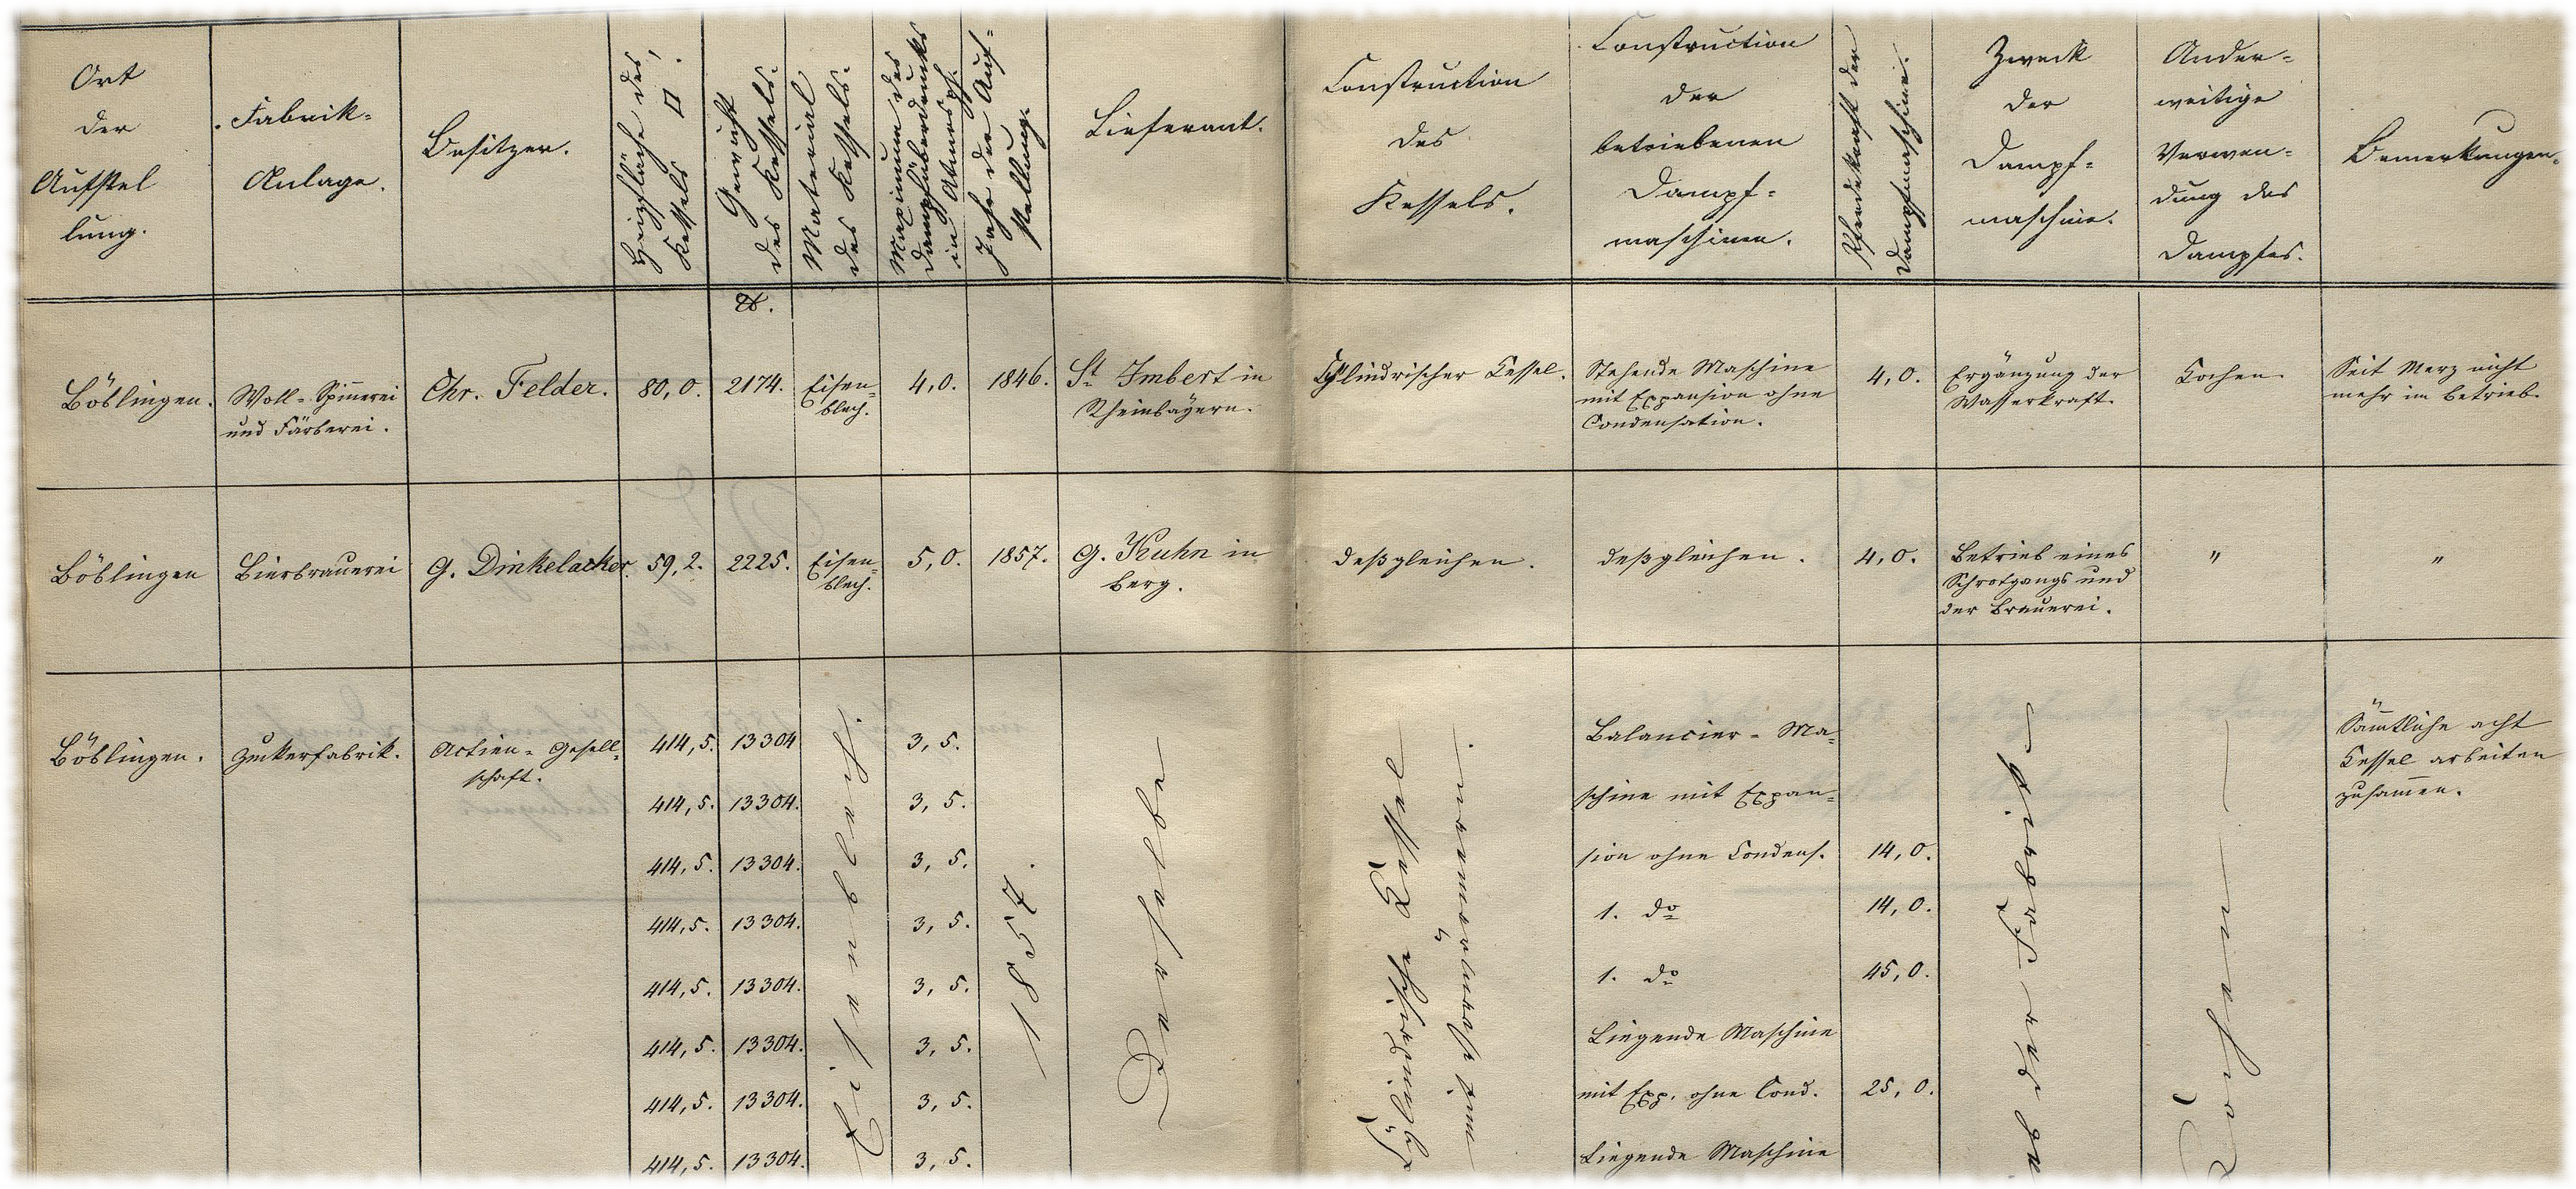
\includegraphics[width=0.7\linewidth]{Steam.png}
    	\end{center}}
    \column{0.5}
    \block{Demographic Change}{
    \begin{itemize}
    	\item The dataset’s \textbf{primary sources are medical statistics and handwritten reports}, regarding deaths, births, and demographic movement, published annually by Württemberg’s \emph{Medizinalkolleg}.
    \end{itemize}

		We approach digitizing these sources by: (1)
		
			\includegraphics[width=0.6\linewidth]{demog.jpg}    
}

\end{columns}

\begin{columns}
	\column{1}
	\block{Follow us!}{
		\begin{center}

		\textbf{We are open to any questions, discussion and feedback!}
		\\
		\vspace{5mm}
		\textbf{Timur Öztürk} \hspace{1cm} \textbf{Prof. Sebastian Braun} \hspace{1cm} \textbf{VWL VII} \vspace{5mm}
		
		\hspace{1.28cm} \includegraphics[height=3cm]{ozturk.png} \hspace{6.5cm} \includegraphics[height=3cm]{braun.png} \hspace{5.5cm} \includegraphics[height=3cm]{vwl7.png} \vspace{8mm}
		\\
	 Financial support from the Deutsche Forschungsgemeinschaft (DFG,471335227) is gratefully acknowledged.
		\end{center}}
\end{columns}

\end{document}